\documentclass{article}

\usepackage{tabularx}
\usepackage{booktabs}
\usepackage{graphicx}
\usepackage{float}

\title{Reflection Report on \progname}

\author{\authname}

\date{}

%% Comments

\usepackage{color}

\newif\ifcomments\commentstrue %displays comments
%\newif\ifcomments\commentsfalse %so that comments do not display

\ifcomments
\newcommand{\authornote}[3]{\textcolor{#1}{[#3 ---#2]}}
\newcommand{\todo}[1]{\textcolor{red}{[TODO: #1]}}
\else
\newcommand{\authornote}[3]{}
\newcommand{\todo}[1]{}
\fi

\newcommand{\wss}[1]{\authornote{blue}{SS}{#1}} 
\newcommand{\plt}[1]{\authornote{magenta}{TPLT}{#1}} %For explanation of the template
\newcommand{\an}[1]{\authornote{cyan}{Author}{#1}}

%% Common Parts

\newcommand{\progname}{ProgName} % PUT YOUR PROGRAM NAME HERE
\newcommand{\authname}{Team \#, Team Name
\\ Student 1 name and macid
\\ Student 2 name and macid
\\ Student 3 name and macid
\\ Student 4 name and macid} % AUTHOR NAMES                  

\usepackage{hyperref}
    \hypersetup{colorlinks=true, linkcolor=blue, citecolor=blue, filecolor=blue,
                urlcolor=blue, unicode=false}
    \urlstyle{same}
                                


\begin{document}
	
	\maketitle
	
	% \plt{Reflection is an important component of getting the full benefits from a
		% learning experience.  Besides the intrinsic benefits of reflection, this
		% document will be used to help the TAs grade how well your team responded to
		% feedback.  In addition, several CEAB (Canadian Engineering Accreditation Board)
		% Learning Outcomes (LOs) will be assessed based on your reflections.}
	
	\section{Changes in Response to Feedback}
	
	% \plt{Summarize the changes made over the course of the project in response to
		% feedback from TAs, the instructor, teammates, other teams, the project
		% supervisor (if present), and from user testers.}
	
	% \plt{For those teams with an external supervisor, please highlight how the feedback 
		% from the supervisor shaped your project.  In particular, you should highlight the 
		% supervisor's response to your Rev 0 demonstration to them.}
	
	\subsection{SRS and Hazard Analysis}
	
	Changes made in response to TAs comment:
	
	\begin{enumerate}
		\item Incomplete Definitions and Formatting: Provided more thorough definitions and changed the formatting of certain words like latex to LaTeX
		\item Organization: Moved the Terminology section to the top of the Project Drivers to provide better clarity. 
		\item Context Diagram: Created a digital context diagram rather than the hand drawn one to improve readability and make it more professional. 
		\item Use Case Diagram: Modified the use case diagram to make some corrections, like removing any internal actors and any unnecessary includes and excludes. Also increased the zoom on the draw.io export to improve readability. 
		\item Functional Requirements: Added rationale for their corresponding functional requirement rather than a separate section. Improved the math specification for the required functional requirements to make it more clear. Abstracted some functional requirements to avoid it being too granular. 
		\item Non-Functional Requirements: Added several more fit criterion to NFRs to provide clear goals to achieve it. Removed any redundancies or contradictions of NFRs with the assumptions being made. 
		\item Reference: Added an external reference in the appendix for the information we required for the project and removed any previous references to draw.io in the doc. 
	\end{enumerate}
	
	\noindent Changes made in response to Peers comment:
	
	\begin{enumerate}
		\item Updated the context diagram to improve clarity. 
		\item Provided detailed rationales for requirements that aren't obvious. 
		\item Improved some requirements that were too detailed or incorrect and made it abstract. 
	\end{enumerate}
	
	\subsection{Design and Design Documentation}
	
	Changes made in response to TAs comment:
	
	\begin{enumerate}
		\item System Context Diagram was added and the project overview section was filled with the necessary information.
		\item Table of Abbreviations and Acronyms in system design document was changed to contain all necessary entries, and is now sorted alphabetically
		\item Timeline in system design document was updated to also reflect our testing plan
		\item Unlikely changes section in MG filled in, difference between project creation and new project modules clarified, type of module information added to all modules, and data related modules moved to software decision modules section.
		\item Minor grammar and spelling issues fixed, and a reference to table 2 added in Connection Between Requirements and Design.
		\item Module decomposition table filled in to match the module guide, and MIS fixed for PDF module, File Services module, Chat module, and File Database Interface module.
		\item Modified a lot of the syntax in the MIS to address issues such as ending module's name with ``Module'', using correct quotations, changing multiple transitions to be simultaneous assignments.
	\end{enumerate}
	
	\noindent Changes made in response to peers comment:
	
	\begin{enumerate}
		\item Fixed the ID of modules to match that of the MG
		\item Added more information about when exceptions are triggered and how the transitions happen for the MIS for some of the modules.
	\end{enumerate}
	
	\noindent Changes made in response to user testing:
	
	\begin{enumerate}
		\item After usability testing conducted with users, the team found out the users rated the applications responsiveness terribly. Further analysis of the walk-through showed that the users were displeased by the loading time when opening files and projects. To fix this delay, the team had to change the current design. Opening new projects took a significant amount of time as the files from GitHub had to be downloaded and entries related to the project had to be created in the database. To resolve this issue, the team decided to move this setup process to when the project is imported rather than when it is opened. From a user perspective, this seemed more acceptable that there was more loading time when importing a project than when opening a project that was already imported. The impact of this change was clearly visible when during the revision 1 walk-through users were not bothered by the opening time.  Large files were taking time to load due to the syntax highlighting used for the editor. There were no quick solutions to this problem, thus the team decided to swap out the editor library(Quill) to a different one(CodeMirror) that was optimized for syntax highlighting. This change resulted in an improvement from 1 min to 2 seconds to open a relatively large file. This upgrade also reflected in a higher responsiveness rating during our revision 1 usability testing.
		\item During user testing we identified some issues with the UI specified in the system design documents. For example, combining UI for import and new project into a single modal was extremely non-intuitive. Likewise having fixed sizes for the PDF renderer, editor, chat, and file menu was also tedious. Thus we updated our UI in the final product to separate the modals for create and import projects and allowed users to have the ability to resize the sub-components on the editor page.
	\end{enumerate}
	
	\subsection{VnV Plan and Report}
	
	Changes made in response to TAs comment:
	
	\begin{enumerate}
		\item Addressed punctuation and grammatical errors 
		\item Fixed conventions of words such as LaTeX and Git to be uniform and correct throughout the document and updated the abbreviations table by removing definitions
		\item Updated the purpose of the VnV to include that that the requirements to be followed are correct and added a document introduction to the VnV report
		\item Added key details to VnV plan pertaining to specific testing methods, roles, evaluation techniques and testers
		\item Adjusted test cases to take in more descriptive input such as a specific file name instead of "enter a new file name", updated output to be correctly defined
		\item Added edge cases to tests and missing tests, such as entering a non-alphanumeric project name
	\end{enumerate}
	
	\noindent Changes made in response to Peers comment:
	
	\begin{enumerate}
		\item Added details about testing methods and roles to VnV plan
		\item Updated usability survey questions to be less ambiguous and include indicators for the scale values
		\item Added missing tests and results
	\end{enumerate}
	
	\noindent Changes made in response to user testing:
	
	\begin{enumerate}
		\item Added additional edge test cases such as hitting the enter key in the chat
	\end{enumerate}
	
	\newpage
	
	\section{Design Iteration (LO11)}
	
	% \plt{Explain how you arrived at your final design and implementation.  How did
		% the design evolve from the first version to the final version?} 
	
	Since the team was developing an application that highly depends on the user experience. We wanted to incorporate some of the principles from user centered-design. We tried to follow an implementation cycle as described in the image below. \\
	
	\begin{figure}[H]
		\centering
		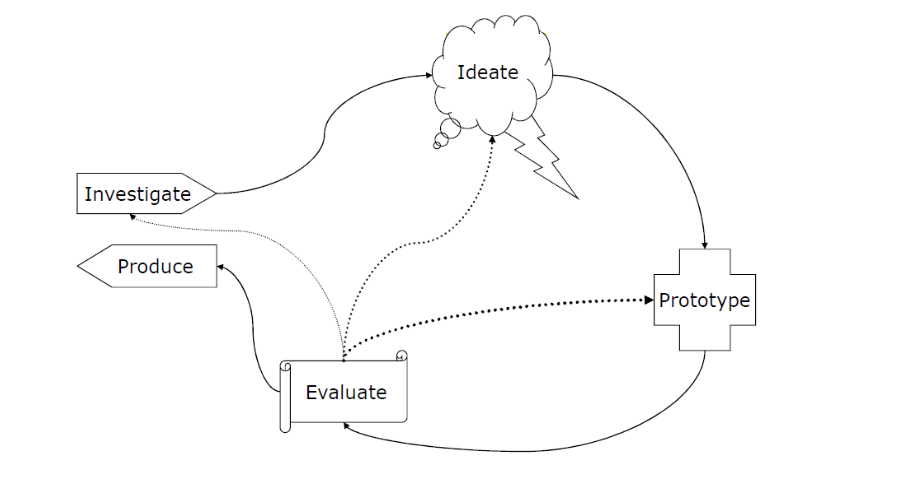
\includegraphics[scale=0.7]{ucd.png}
		\caption{User Centered Design Cycle}
	\end{figure}
	
	\subsection{Investigate}
	The first stage in this cycle is where the team learnt about stakeholders, discovered their needs and goal with respect to UnderTree. The team was able to come up with use cases and all the requirements for the project
	\subsection{Ideate}
	Ideate is the stage where we went from our requirements to our design details such as coming up with the modules, their functionality and their relationship between each other.
	\subsection{Prototype}
	Prototype was the stage where we implemented all of functionalities into revision 0 of the application. These functionalities were based of the functional and non-functional requirements that the team came up with in the previous stages. \\\\
	During implementation, the team also found that requirements originally specified were not able to match the new implementation. Therefore, the requirements had to be edited to better support our the new findings gained during implementation. There were cases where it came to note some of the modules can be merged into a single modules. Those changes also had to be reflected in our design documentation, thus those were also edited.
	\subsection{Evaluate}
	In this stage, we tested revision 0 of the application within 3 categories which are requirements evaluation, unit testing and usability testing.
	
	\subsubsection{Requirements Evaluation}
	Requirements evaluation consisted of manually testing functional requirement and non functional requirements. This type of evaluation allowed the team to notice requirements that the team might have failed to implement. One such example is test ST-15 which check if the editor highlights spelling error the user makes while editing the latex file. This test failed as there was no implementation done for spell check as it proved rather challenging to implement within the project deadline. The team then concluded that this requirement corresponding to this test, FR23 should be dropped as it is not feasible.
	
	\subsubsection{Unit Testing}
	
	Unit testing was set up for crucial backend modules such as Project, File, Chat and Auth services. Unit tests allowed us discover smaller issues that cannot be found by just doing requirement evaluation. It also allowed us regressions that may be created when a change is made. One such example is the unit test-case of FS-4. This test started failing after some refactoring was done to the editor module in the client. This test case allowed us to identify the issue with the change made to editor, thus a fix was quickly produced to make sure the scenario that the unit test was accoutable for could pass again.
	
	\subsubsection{Usability Testing}
	
	Usability testing was the most important testing done by the team since our application is highly user experience focused. Usability testing was done through using use-task walk-through combined with a survey at the end of the walk-through. Use-task walk-through are just activities where users go through a set of provided scenarios, while the walk-through supervisors take note of the pain points and actions that the users do differently than intended. Through the survey results, the team reached the conclusion that the current user interface was not very intuitive and the application was slow. The walk-through was also analyzed to take notes of the feature that can be made more intuitive.
	
	\subsection{Produce}
	
	Finally, in this stage, the team produced revision 1 of the application which incorporated most of the feedback from all the stakeholders. This version was also re-evaluated with users using the same testing methods as previously mentioned. As expected, the intuitiveness rating and responsiveness rating for UnderTree went up drastically due to the changes that were made. Although this project is stopping at revision 1, this process will cycle back to reevaluation, go through previous stages and produce a new version of the application.
	
	\section{Design Decisions (LO12)}
	
	\subsection{Time}
	
	\noindent The biggest limitation we faced when we first started designing this system was time. As this is a relatively large project with multiple subsystems that can be implemented separately, we decided to make use of as many existing libraries and solutions as possible. This was a design decision made early on so that we could accomplish everything we intended to within the given time limit.\\
	
	\noindent Guided by the fact that we did not have the necessary expertise to build a secure login and authentication system from scratch, we made the decision to use GitHub as our version control and authentication system. However, this decision came with a lot of constraints since we had to guide our system around what was allowed by the GitHub API. Despite this, we were able to modify our requirements to work around these constraints, and since we made this decision early on, it was relatively simple to do so.\\
	
	\noindent We also chose to use JavaScript as both our front-end and back-end language since we were most familiar with it, and it had a vast number of libraries to support and speed up the development time, which was necessary to meet the time constraint. However, we acknowledged that a language like Go or Rust would be better suited for the multi-threaded needs of our system.
	
	\subsection{Expertise}
	
	During the development of our project, we encountered specific subsystems that required knowledge and expertise outside of our team's skill set. These subsystems included authentication using JSON Web Tokens (JWT), integrating with GitHub using OAuth and webhooks, and implementing synchronization algorithms such as operational transformation and Conflict-free Replicated Data Types (CRDT) for enabling real-time multi-user edits to documents. Though after a bit of research we were able to quickly figure out how to correctly implement JWTs and GitHub OAuth with our systems, despite spending much of the time before the POC demo on the synchronization algorithm, we were not able to account for the various edge cases that the implementation needed to consider. Though on the surface these algorithms are relatively robust, implementing them perfectly required a high level of expertise and time to understand and read through multiple research papers which we did not have. As a result, we decided to use yjs, an existing CRDT library to handle the synchronization for us. This imposed specific constraints on how documents had to be saved in our database and server which required a bit of modification to our system to integrate, however these modifications were still simpler than taking time to develop the expertise to implement these algorithms correctly. This time spend researching these algorithms was not wasted though, as it helped us develop a better understanding of the differences between the algorithms and to determine that CRDT was a better fit for our system due to its higher speed and offline capabilities.\\
	
	\noindent During the development of our project, we faced another expertise limitation with web sockets. We needed to establish a reliable and efficient communication channel between the client-side and server-side components of our system in order to facilitate real-time collaboration, and messaging. However, web sockets can be challenging to implement and require a deep understanding of the underlying protocols and technologies. To address this limitation, we decided to use the Socket.IO library, which provides a high-level, easy-to-use API for working with web sockets. Socket.IO abstracts away many of the complexities of working with web sockets and provides a simple interface for sending and receiving real-time messages between the client and server. With Socket.IO, we were able to quickly and easily set up a real-time communication channel between our client and server components, without needing to spend significant time and effort on low-level socket programming.
	
	\subsection{Cost}
	
	Though it would have been optimal to host our system on a well established and easy to scale service like AWS, it would have been extremely costly to do so. This is because, due to the constant communication required between clients for the real-time editing and chat messaging aspects of our system, we would not be able to utilize the cost-effective server-less products such as lambda that AWS provides. Using a service like amplify would have been significantly more expensive and not some that we would be able to afford. Thus we had to make the decision to move completely away from the AWS ecosystem and deploy our project manually on bare bones servers that we would rent from sites like digital ocean. Due to this decision we had to take time to learn about devops and how to securely deploy a web application using docker and nginx/caddy.
	
	\section{Economic Considerations (LO23)}
	
	During our testing and after receiving user feedback, we discovered a strong interest in our project. We determined that our target market would mainly consist of students and researchers, although an extensive research was not conducted to determine the size of this market. We identified at least 17 potential users, most of whom are Software Engineering students like us. Since our project is intended to be open source, we don't need to sell any units or meet a minimum user threshold to make a profit. Advertising can be simplified by posting about it on social media platforms such as LinkedIn and Reddit, and we can also promote it through word of mouth to students at McMaster University, who would be interested in using it. If we were to make this system a paid service, it would likely discourage many existing users who value its open-source nature. As a result, most of the funds required to offset the cost of hosting this service would need to come from donations or by offering premium features that could be implemented in the future.
	
	\noindent It would be worthwhile to do some level of market research to help us better identify how big our actual market is and how to more effectively advertise to them aside from the basic methods listed above.
	
	\section{Reflection on Project Management (LO24)}
	
	\subsection{How Does Your Project Management Compare to Your Development Plan}
	
	% \plt{Did you follow your Development plan, with respect to the team meeting plan, 
		% team communication plan, team member roles and workflow plan.  Did you use the 
		% technology you planned on using?}
	
	\subsubsection{Meeting plan}
	
	The meeting plan specified in the development plan was about meeting twice a week. The team did have to make changes to this meeting plan. As the project progressed, the team noticed there was no need to meet that frequently as there was not much updates or issues to discuss about. The new meeting plan was once per week, and more frequent when a deadline for a deliverable was approaching. This drastically improved our productivity as we were spending less time in meetings and more time working on the deliverable or implementation.
	
	\subsubsection{Team communication plan}
	
	The team communication plan also evolved during the course of the project. Originally, meetings were planned to be held in person but it became apparent that scheduling everyone for an in person meeting was difficult, thus online meeting became the default. It also became more evident that asynchronous communication is more efficient for our project that having to get everyone to meet for discussion. For example, if someone has a problem with some code, they do not need to wait till some meeting but rather could just message the team about it. Whoever is available can then respond to the message. Although asynchronous communication was encourages, there was some benefit of synchronous communication too. Some of the members used the meeting as motivation to complete their work by thus it definitely helped with productivity in certain situations.
	
	\subsubsection{Team member roles}
	
	Our team member roles relatively stayed the same. The only change that was made was made was that Faiq who was the domain expert of Rust had to take on the role of being the domain expert of Typescript and Node.js. This change happened due to the fact that the team switched to using Node.js for the backend instead of Rust.\\
	
	\subsubsection{Workflow Plan}
	
	The team stuck to the original workflow plan of using branches to implement new features and merging them to main. We found this strategy was very efficient and productive. Even if the feature some other team member is working is not complete yet, one is able to continue one with their own work in their branch. We did not use Zenhub for issue tracking as originally mentioned in the development plan.
	
	
	\subsection{What Went Well?}
	
	Firstly, using multiple branches really helped us succeed in being efficient in our development and deployment. One such example is that it allows to continue development before a demo because it would not put the application in a bad state as the changes would be in a different branch and the main branch can be used for the application that will be deployed. Using branches also enabled the team to use pull requests. Pull requests were very beneficial to ensuring team members were pushing code that was not going to conflict, and also allowed us re-iterate and write better code.
	
	\subsection{What Went Wrong?}
	
	One of the issue that existed withing our team was that we were inefficient and disorganized at tracking tasks. One of the main reason might be that we were not using a specific issue tracking/ project management tool but rather depending on GitHub issues. We were also not enforcing tracking tasks through issues. What this meant for the team was that a lot of the time, tasks that were to be done are lost, and never worked on. One such example is that there is a bug where the document synchronized in the editor is not deleted once a project is deleted. The team found this issue early on but lost track of it. Not fixing till later added high priority tasks right before deadlines for revision 1 demo. If this bug was tracked as an issue from the start, it would have easily been fixed earlier in development. Not tracking issues also leads to another problem where team members have to be constantly reminded on the tasks that need to be done. If these tasks were created from the start with assigned developers, it would also help the developers know what they have to work on next.
	
	\subsection{What Would you Do Differently Next Time?}
	
	For the next time, we would try to use an issue tracking software such as ZenHub and enforce the creation of issues and bugs. This will ensure the team does not lose tasks that need to be done and will also keep each of the team member in track.
	
\end{document}